\documentclass{article}[12pt]
\usepackage[a4paper, margin=1in]{geometry}
\usepackage{amsmath}
\usepackage{graphicx}

\begin{document}

\section*{Exercícios}

\begin{enumerate}
    \item Obtenha a tabela-verdade a partir das expressões:
    \begin{enumerate}
        \item $S = \overline{AB}C + A\overline{BC} + A\overline{B}C + ABC + AB\overline{C} + ABC$ \\
        \textbf{R.:}
        \begin{center}    
            \begin{table}[h]
                \label{tab:2a}
                \begin{tabular}{|p{0.8cm}|p{0.8cm}|p{0.8cm}|p{0.8cm}|p{0.8cm}|p{0.8cm}|p{0.8cm}|p{0.8cm}|p{0.8cm}|p{0.8cm}|p{0.8cm}|p{0.8cm}|p{0.8cm}|}
                    \hline
                    \(\mathbf{A}\) & \(\mathbf{B}\) & \(\mathbf{C}\) & \(\mathbf{\overline{A}}\) & \(\mathbf{\overline{B}}\) & \(\mathbf{\overline{C}}\) & \(\mathbf{\overline{A}B\overline{C}}\) & \(\mathbf{A\overline{B}\overline{C}}\) & \(\mathbf{A\overline{B}C}\) & \(\mathbf{ABC}\) & \(\mathbf{AB\overline{C}}\) & \(\mathbf{\overline{A}BC}\) & \(\mathbf{S}\) \\ \hline
                    0 & 0 & 0 & 1 & 1 & 1 & 0 & 0 & 0 & 0 & 0 & 0 & 0 \\ \hline
                    0 & 0 & 1 & 1 & 1 & 0 & 1 & 0 & 0 & 0 & 0 & 0 & 1 \\ \hline
                    0 & 1 & 0 & 1 & 0 & 1 & 0 & 0 & 0 & 0 & 0 & 0 & 0 \\ \hline
                    0 & 1 & 1 & 1 & 0 & 0 & 0 & 0 & 0 & 0 & 0 & 1 & 1 \\ \hline
                    1 & 0 & 0 & 0 & 1 & 1 & 0 & 1 & 0 & 0 & 0 & 0 & 0 \\ \hline
                    1 & 0 & 1 & 0 & 1 & 0 & 0 & 0 & 1 & 0 & 0 & 0 & 1 \\ \hline
                    1 & 1 & 0 & 0 & 0 & 1 & 0 & 0 & 0 & 0 & 1 & 0 & 1 \\ \hline
                    1 & 1 & 1 & 0 & 0 & 0 & 0 & 0 & 0 & 1 & 0 & 0 & 1 \\ \hline
                \end{tabular}
            \end{table}
        \end{center}

        \item $S = A\overline{B} + ACD + A\overline{B}C$ \\
        \textbf{R.:} 
        \begin{center}
            \begin{table}[h]
                \label{tab:2b}
                \begin{tabular}{|p{0.8cm}|p{0.8cm}|p{0.8cm}|p{0.8cm}|p{0.8cm}|p{0.8cm}|p{0.8cm}|p{0.8cm}|p{0.8cm}|}
                    \hline
                    \(\mathbf{A}\) & \(\mathbf{B}\) & \(\mathbf{C}\) & \(\mathbf{D}\) & \(\mathbf{\overline{B}}\) & \(\mathbf{A\overline{B}}\) & \(\mathbf{ACD}\) & \(\mathbf{A\overline{B}C}\) & \(\mathbf{S}\) \\ \hline
                    0 & 0 & 0 & 0 & 1 & 0 & 0 & 0 & 0 \\ \hline
                    0 & 0 & 0 & 1 & 1 & 0 & 0 & 0 & 0 \\ \hline
                    0 & 0 & 1 & 0 & 1 & 0 & 0 & 0 & 0 \\ \hline
                    0 & 0 & 1 & 1 & 1 & 0 & 0 & 0 & 0 \\ \hline
                    0 & 1 & 0 & 0 & 0 & 0 & 0 & 0 & 0 \\ \hline
                    0 & 1 & 0 & 1 & 0 & 0 & 0 & 0 & 0 \\ \hline
                    0 & 1 & 1 & 0 & 0 & 0 & 0 & 0 & 0 \\ \hline
                    0 & 1 & 1 & 1 & 0 & 0 & 0 & 0 & 0 \\ \hline
                    1 & 0 & 0 & 0 & 1 & 1 & 0 & 0 & 1 \\ \hline
                    1 & 0 & 0 & 1 & 1 & 1 & 0 & 0 & 1 \\ \hline
                    1 & 0 & 1 & 0 & 1 & 1 & 0 & 1 & 1 \\ \hline
                    1 & 0 & 1 & 1 & 1 & 1 & 1 & 1 & 1 \\ \hline
                    1 & 1 & 0 & 0 & 0 & 0 & 0 & 0 & 0 \\ \hline
                    1 & 1 & 0 & 1 & 0 & 0 & 0 & 0 & 0 \\ \hline
                    1 & 1 & 1 & 0 & 0 & 0 & 0 & 0 & 0 \\ \hline
                    1 & 1 & 1 & 1 & 0 & 0 & 1 & 0 & 1 \\ \hline
                \end{tabular}
            \end{table}
        \end{center}
    \end{enumerate}

    \item Determine a expressão do circuito lógico:
    \begin{enumerate}
        \item
            \begin{figure}[h!bt]
                \begin{center}
                    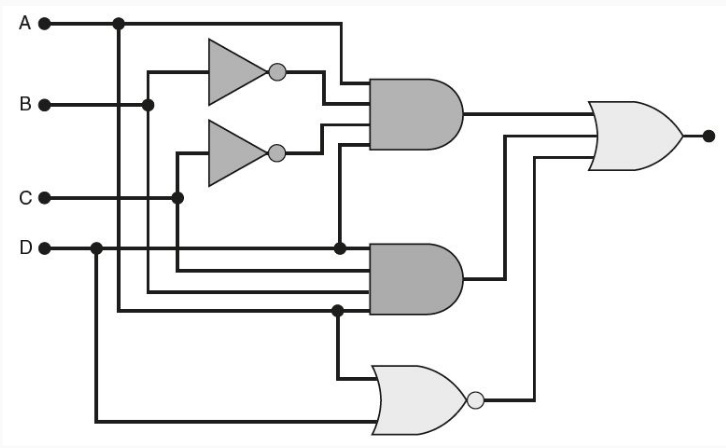
\includegraphics[scale=1]{images/2a.png}
                    \hspace{1cm}
                    $S = (A\overline{BC}D) + (ABCD) + (\overline{A+D})$
                \end{center}
            \end{figure}
        \item
            \begin{figure}[h!bt]
                \begin{center}
                    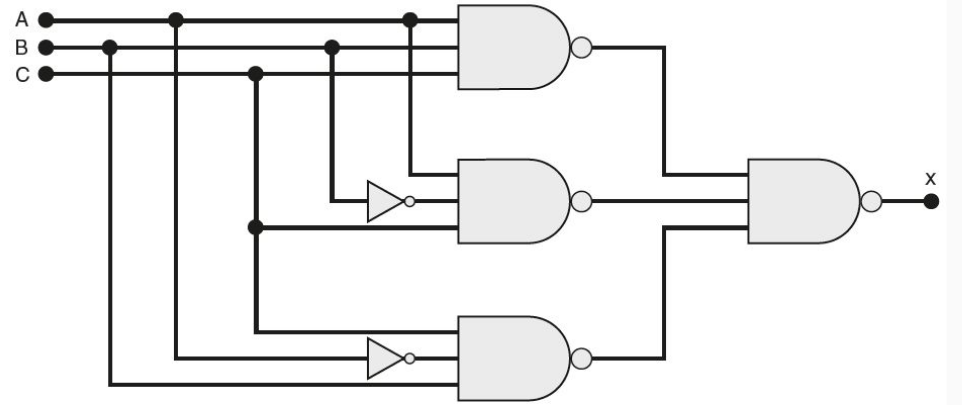
\includegraphics[scale=1]{images/2b.png}
                    \hspace{1cm}
                    $S = \overline{ABC}.\overline{A\overline{B}C}.\overline{\overline{A}BC}$
                \end{center}
            \end{figure}
        \item
            \begin{figure}[h!bt]
                \begin{center}
                    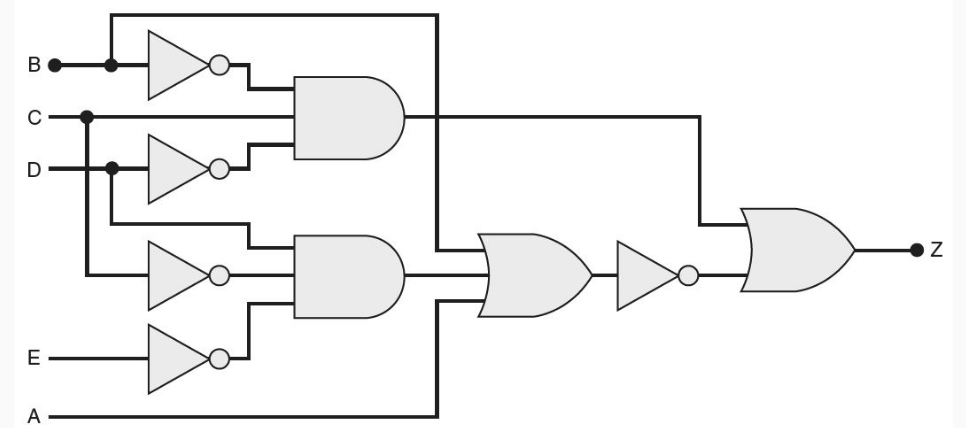
\includegraphics[scale=1]{images/2c.png}
                    \hspace{1cm}
                    $S = (\overline{B}C\overline{D})+(\overline{B+D\overline{CE}+A})$
                \end{center}
            \end{figure}
        \item
            \begin{figure}[h!bt]
                \begin{center}
                    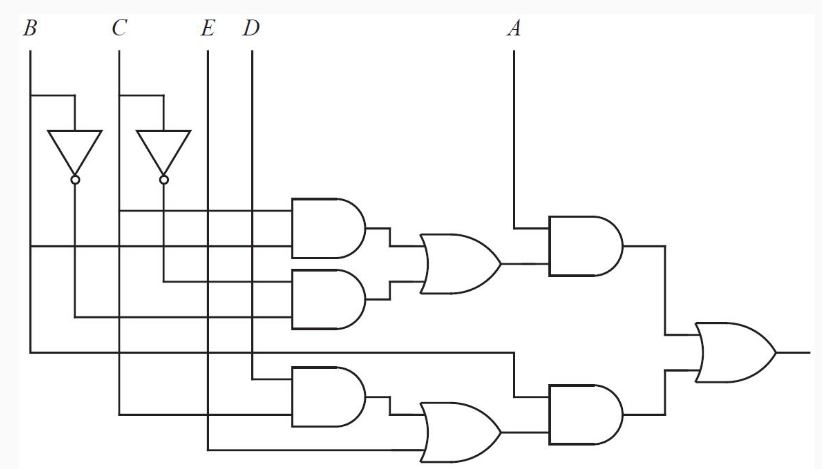
\includegraphics[scale=1]{images/2d.png}
                    \hspace{1cm}
                    $S = (A.CB+\overline{CB})+(B.DC+E)$
                \end{center}
            \end{figure}
    \end{enumerate}

\pagebreak
    \item Desenhe o circuito lógico das expressões:
    \begin{enumerate}
        \item
            \begin{figure}[h!bt]
            \begin{center}
                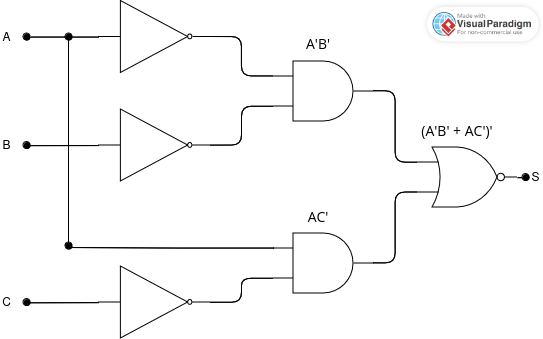
\includegraphics[scale=0.25]{images/3a.png}
                \hspace{1cm}
                $S = \overline{\overline{AB} + A\overline{C}}$
            \end{center}
            \end{figure}
        \item
            \begin{figure}[h!bt]
            \begin{center}
                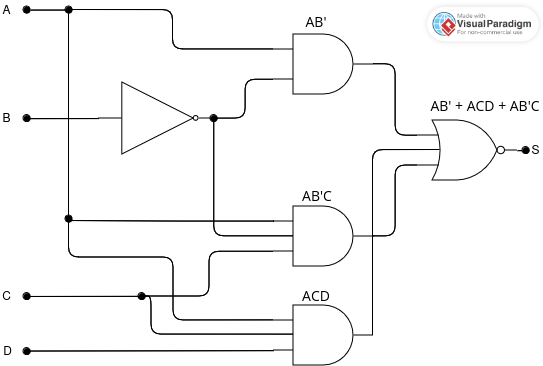
\includegraphics[scale=0.25]{images/3b.png}
                \hspace{1cm}
                $S = A\overline{B} + ACD + A\overline{B}C$
            \end{center}
            \end{figure}
        \item
            \begin{figure}[h!bt]
            \begin{center}
                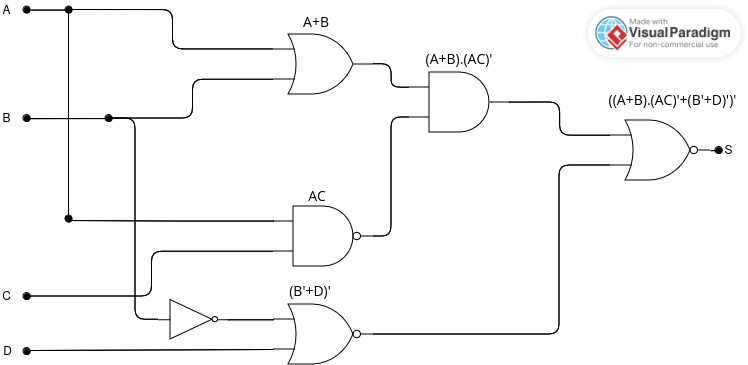
\includegraphics[scale=0.25]{images/3c.png}
                \hspace{1cm}
                $S = \overline{(A+B)\overline{AC} + \overline{(\overline{B}+D)}}$
            \end{center}
            \end{figure}
        \item
            \begin{figure}[h!bt]
            \begin{center}
                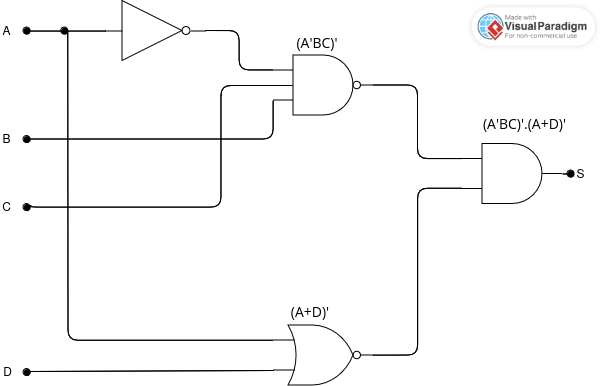
\includegraphics[scale=0.25]{images/3d.png}
                \hspace{1cm}
                $S = \overline{\overline{A}BC}.\overline{(A+D)}$
            \end{center}
            \end{figure}
        \item
            \begin{figure}[h!bt]
            \begin{center}
                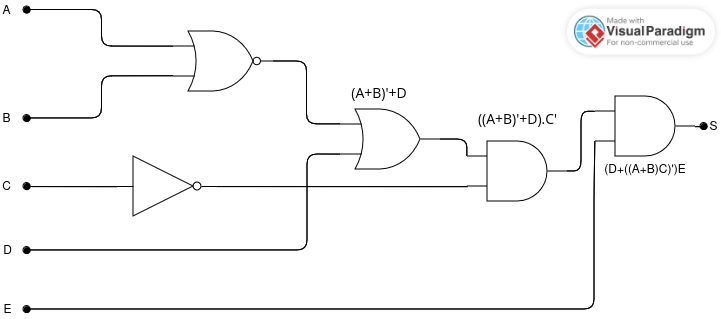
\includegraphics[scale=0.25]{images/3e.png}
                \hspace{1cm}
                $S = (D+\overline{(A+B)C})E$
            \end{center}
            \end{figure}
    \end{enumerate}
\end{enumerate}

\end{document}